\newcommand{\floor}[1]{\lfloor #1 \rfloor}

\begin{problem}{Uninformed Search and Heuristics}

Consider the following simplified version of the classic Atari video game, \textit{Montezuma's Revenge}: It is played on the board illustrated below. An agent (represented by the person icon in cell (1,3)) wishes to grab the key (in cell (3,0)). A skull starts in cell (5,2) and moves to the right by one cell after each action is executed until it ends up in the rightmost cell, at which point it starts moving to the left, and repeats this pattern back and forth. 

The agent can be facing either left or right. There are 10 possible actions for the agent: 2 turning actions ($face\_left, face\_right$) and 8 moving actions ($left, right, up, down, left\_up, left\_down,$ $right\_up, right\_down$). The agent can move up or down while facing either direction, but can move sideways or diagonally only if facing in that direction. For example, if the agent is facing right but tries to move $left\_up$, the agent will not move and nothing will happen. Furthermore, if the agent is already facing $left$ and a $face\_left$ action is taken, nothing happens.

Lastly, the agent cannot move into a cell \textbf{currently occupied} by the skull, or a wall. 


\begin{center}
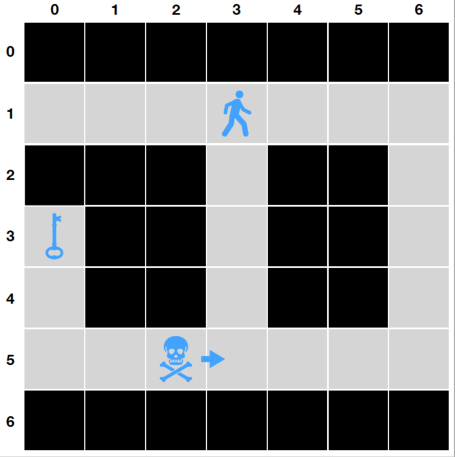
\includegraphics[width=0.3\textwidth]{figures/montezuma_revised.pdf}
\label{fig:montezuma}
\end{center}

\begin{question}
Answer the following questions for the Montezuma's revenge board above:

\vspace{0.1in}

\begin{subquestion}[7]
Let $N$ be the number of possible cell locations that the agent can be in, and let $M$ be the number of possible cell locations that the skull can be in. Recall that for ``pacman pathing", the representation of the state was $(x,y)$ where $x$ was the row and $y$ was the column of pacman's position.  

Describe the minimal state space representation of a state in the state space for this game and give an expression for the size of the state space.\\\\

Representation of the state space:

Size of the state space: 

Explanation of each term in the size of the state space: 

 
\end{subquestion}

\vspace{0.4in}

\newpage
\begin{subquestion}[3]
What is the goal test?


\end{subquestion}
\end{question}

\newpage

\begin{question}
Now, consider the simplified board below, which has \textbf{no skull} and \textbf{no facing-direction for the agent} (i.e., the agent can move in any of the 8 directions as long as it remains in the board). For the three following graph search algorithms, perform the search procedure yourself (\textbf{please show your work}) and provide answers to the questions below regarding the nodes expanded during the search as well as the final path found by the algorithm.

On this board, assume that a diagonal move has a cost of 3, whereas moving left, right, up, or down has a cost of 1. Do notice the difference in costs, and recall which algorithms use this cost information and which algorithms do not.

Remember that the search procedure should begin at the agent's starting position (C). To break ties when adding nodes of equal cost to the frontier, follow alphabetical order; for example, if you are considering nodes B and E with the same cost, then add node B to the frontier ahead of node E.

By convention, the depth of the starting node is 0, and the length of a path is the number of edges it contains.

Finally, when listing the order/number of nodes expanded, do not include nodes which are taken off the frontier but discarded immediately due to already having been expanded.

\begin{center}
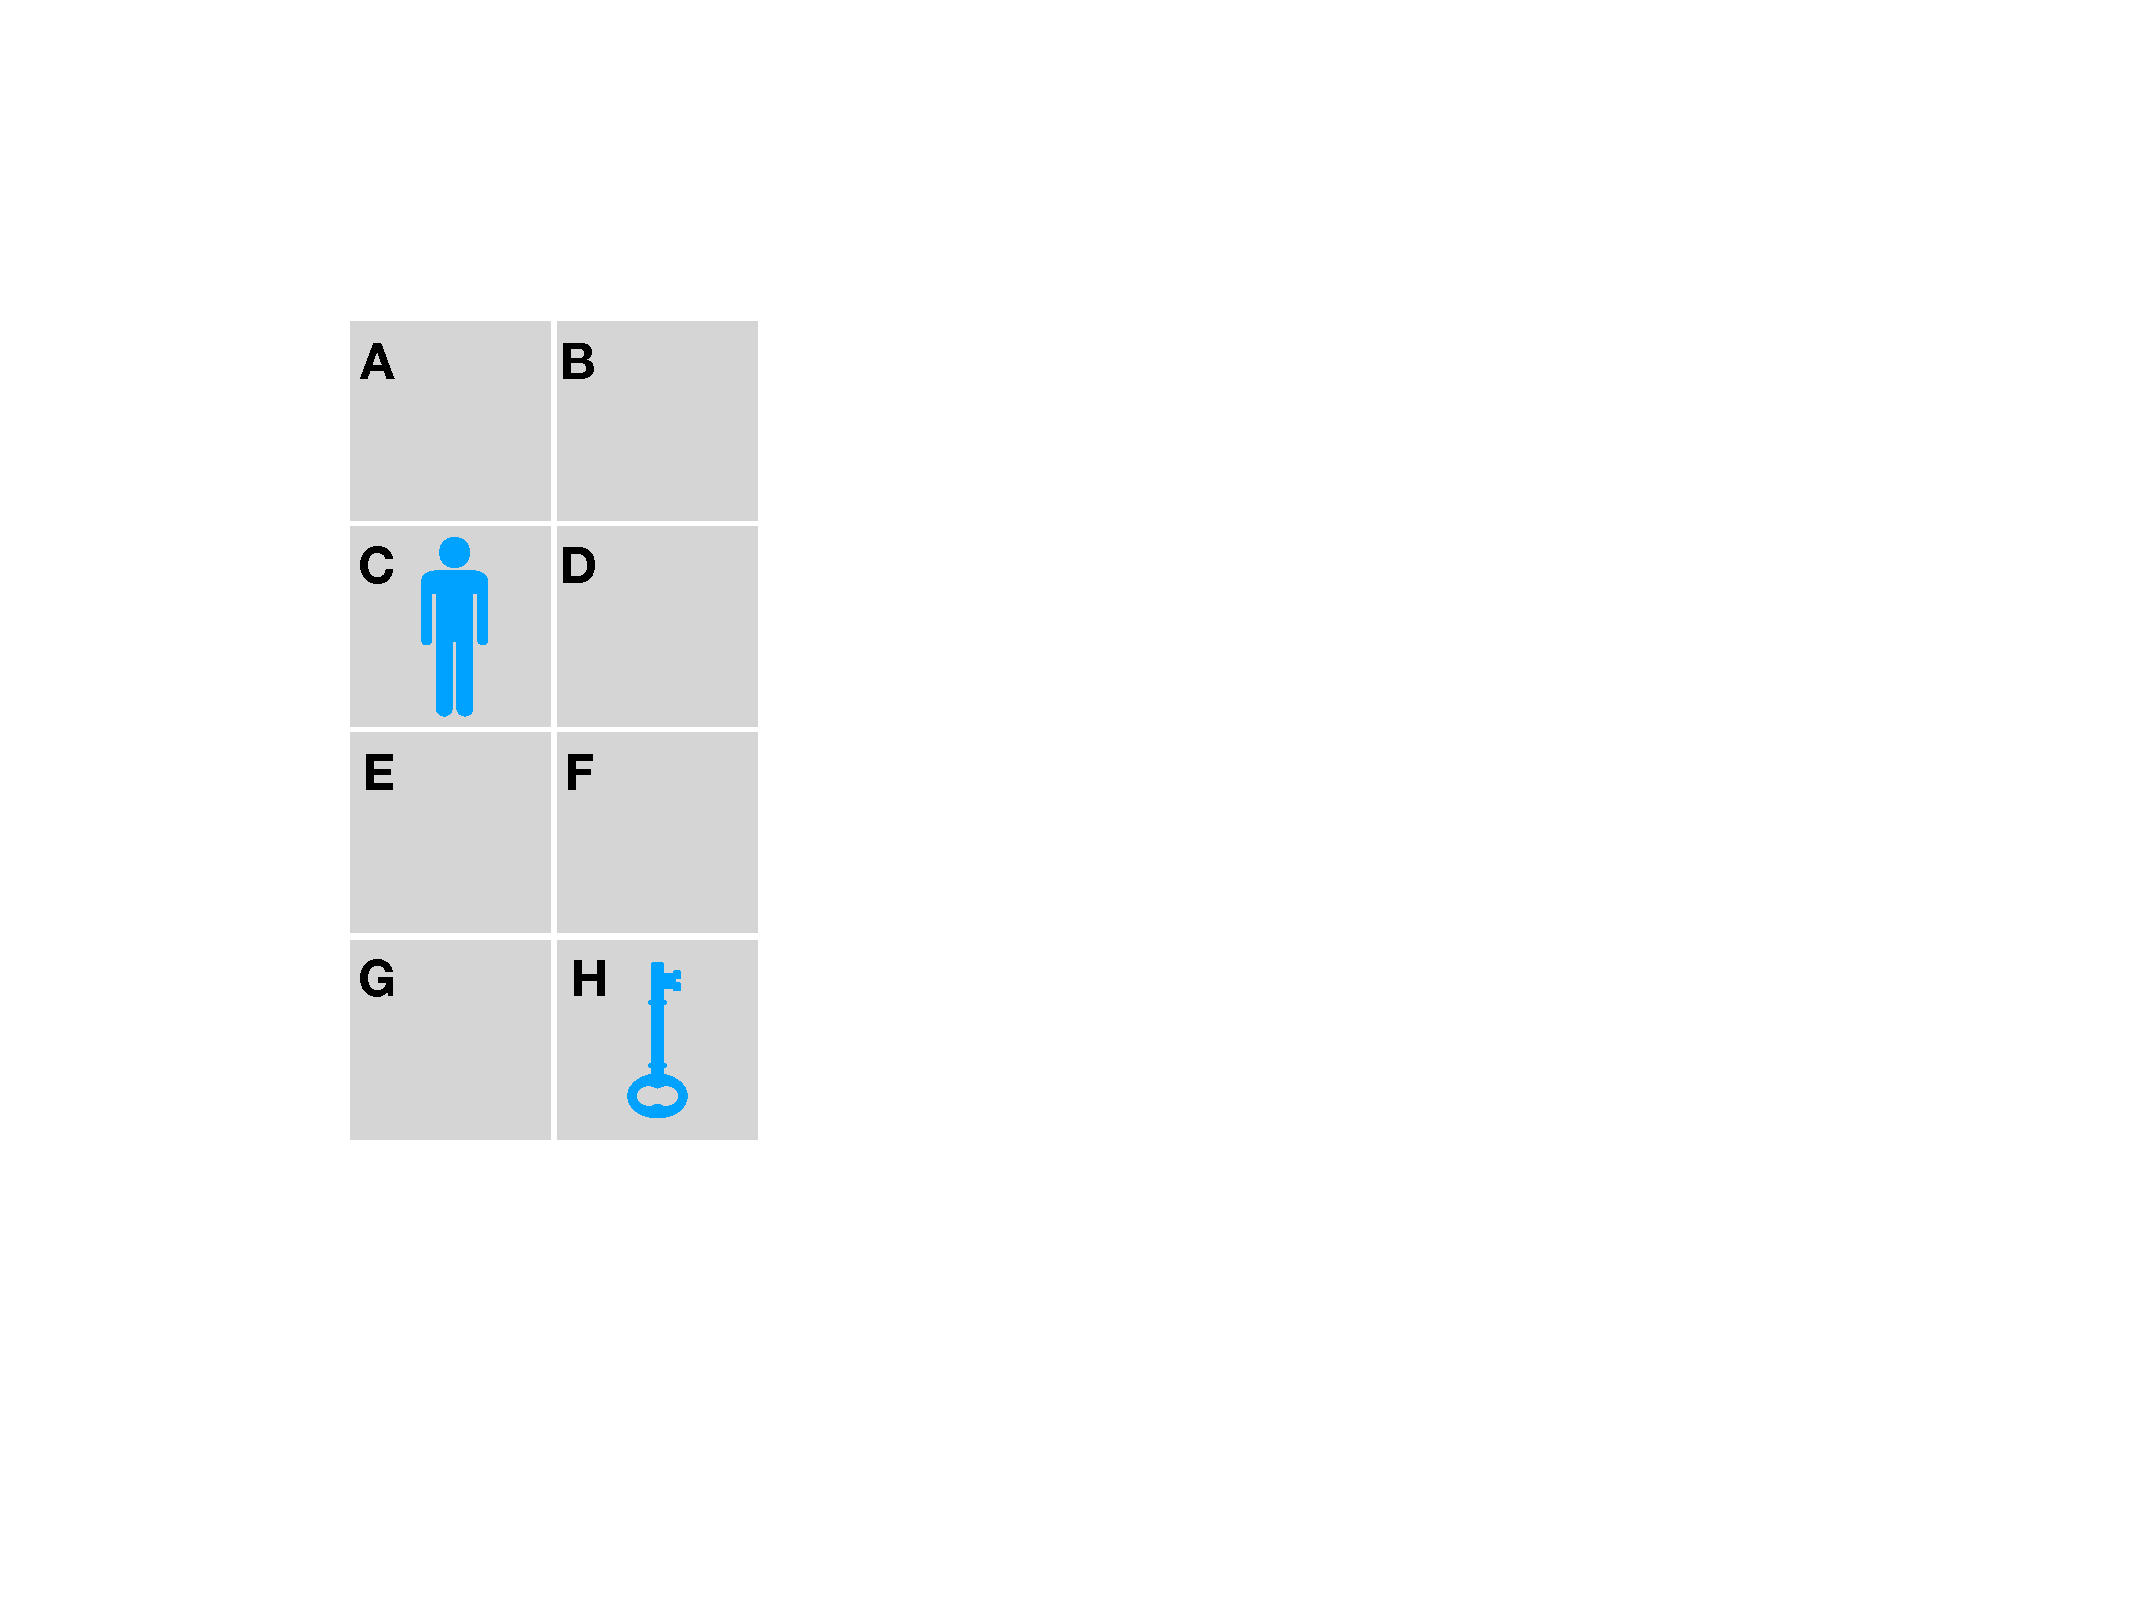
\includegraphics[width=0.15\textwidth]{figures/simple_nodir.pdf}
\label{fig:montezuma}
\end{center}

\newpage
\begin{subquestion}[8]
\textbf{Breadth-first graph search}\\
Frontier data structure: FIFO.\\
Recall that BFS selects the {\em shallowest} unexpanded node in the frontier for expansion, which will be the {\em oldest} node in the frontier.\\

\begin{center}
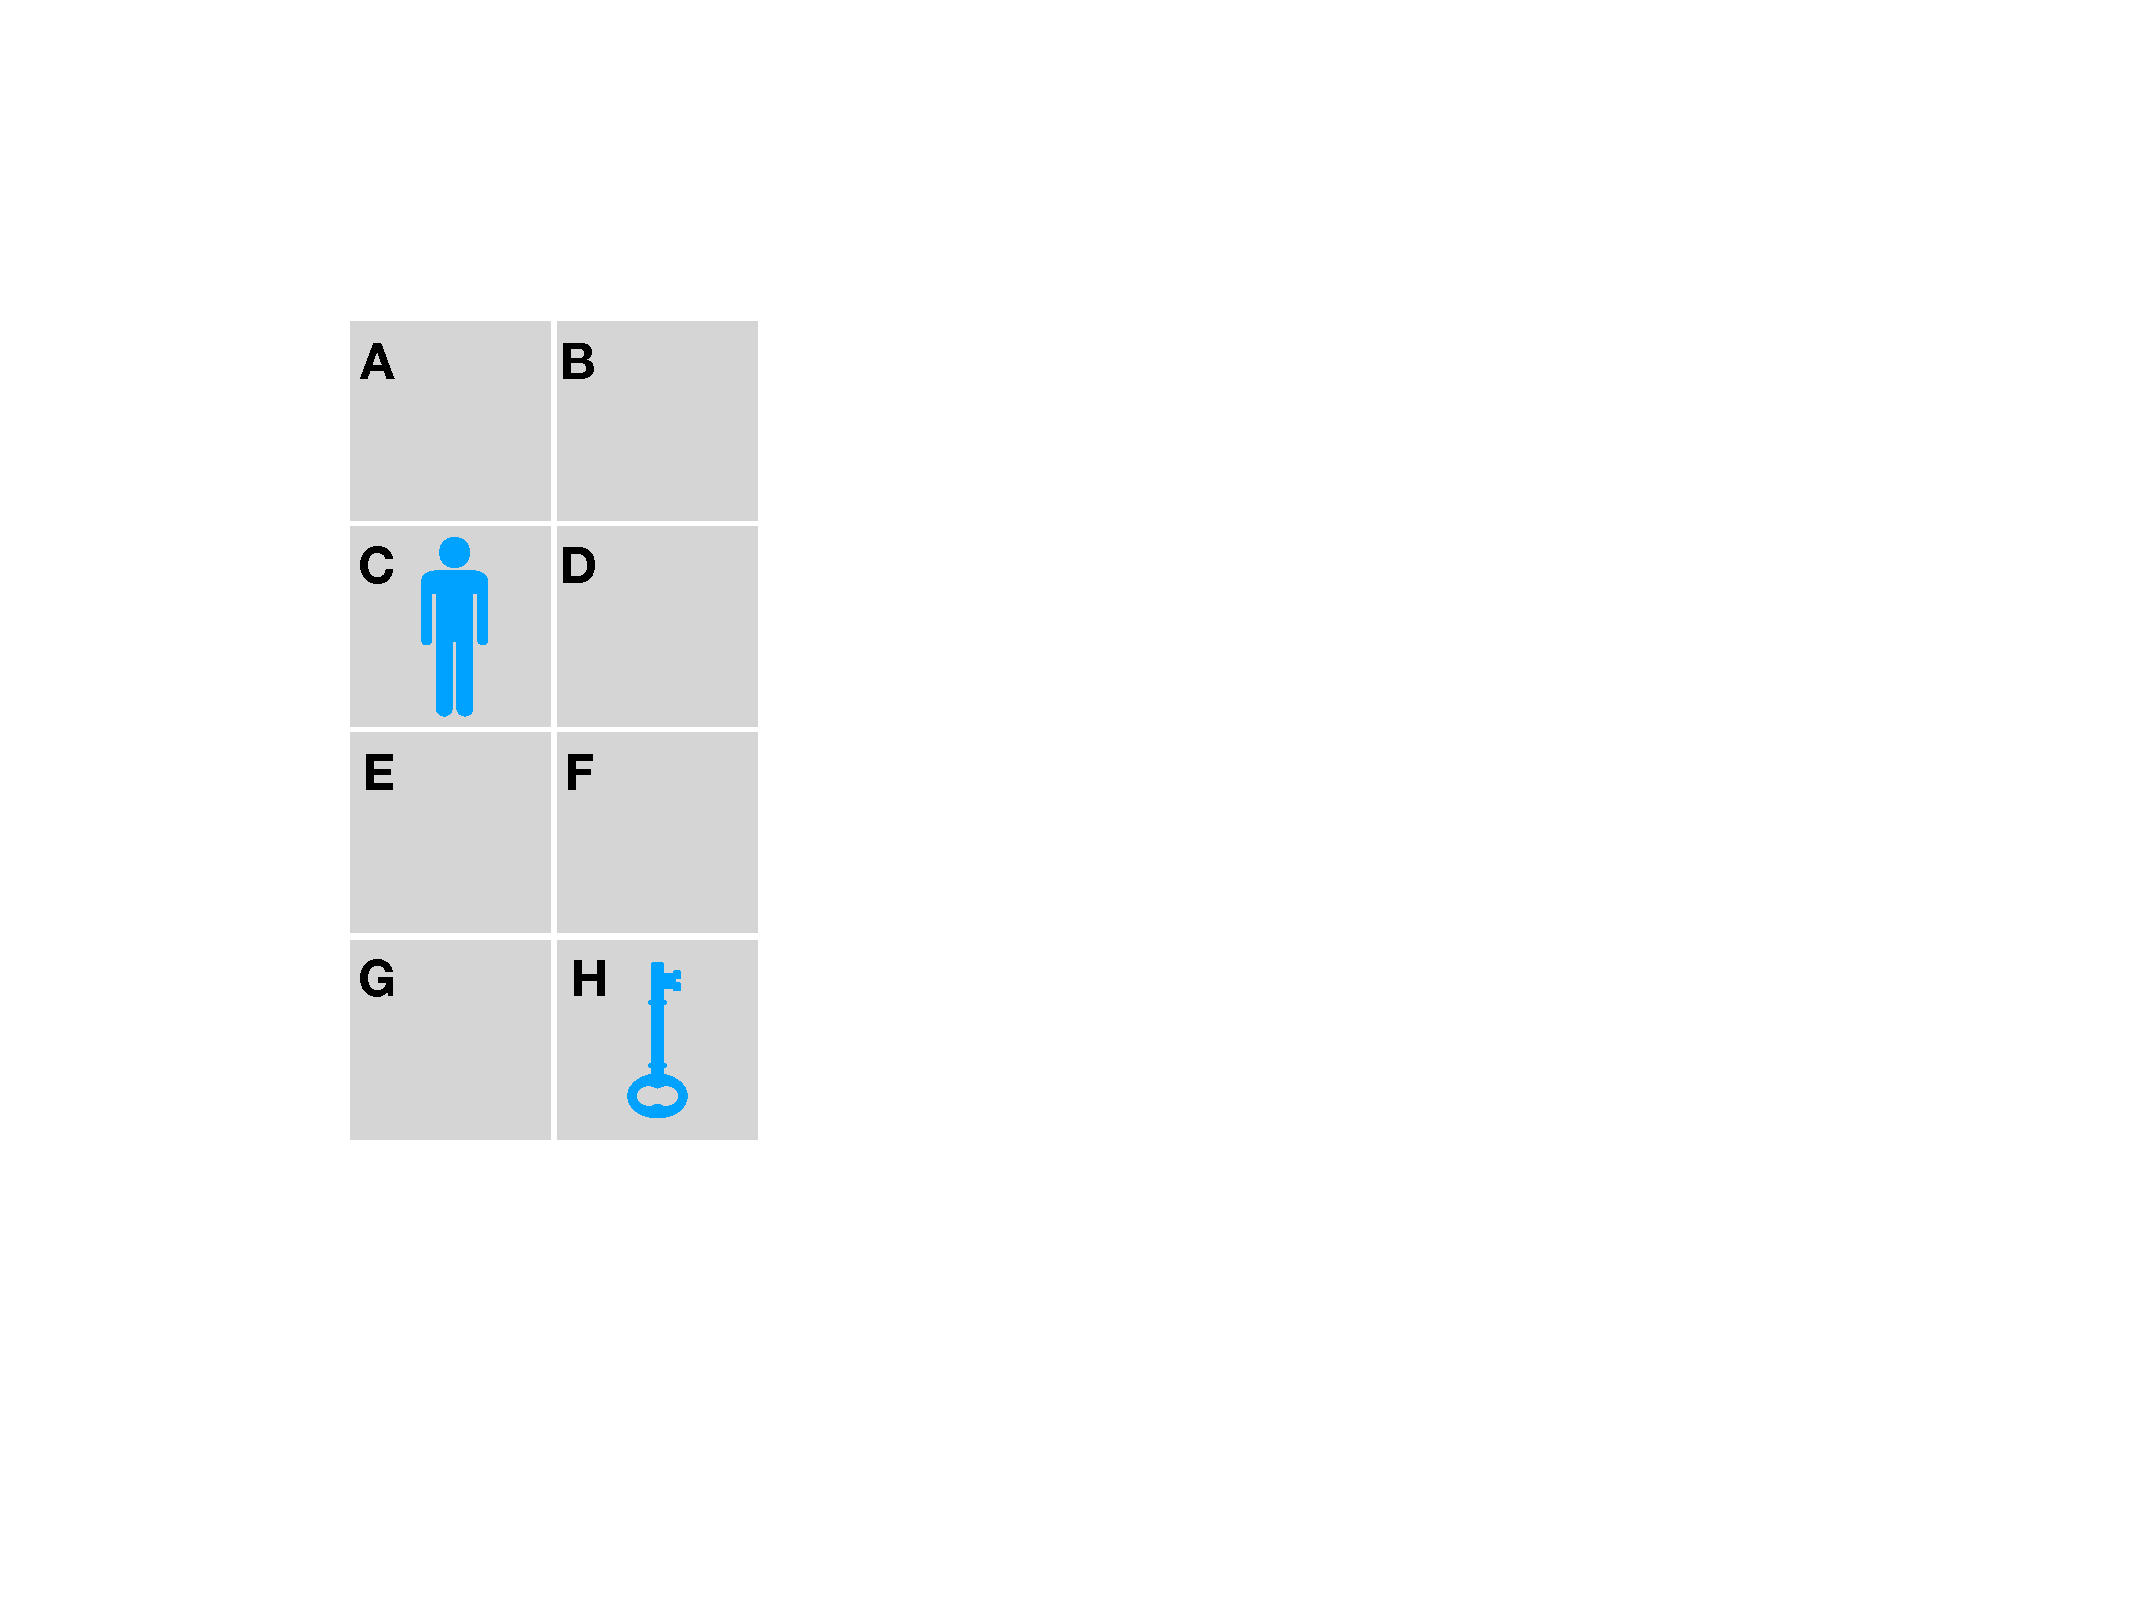
\includegraphics[width=0.15\textwidth]{figures/simple_nodir.pdf}
\label{fig:montezuma}
\end{center}



Order of nodes expanded:

Number of nodes expanded: 

Path returned: 

Length of path: 

Cost of path: 

What are the {\em depths} $d(A), d(B), \ldots d(H)$?

\def\arraystretch{1.5}
\setlength\tabcolsep{15pt}
\begin{center}
\begin{tabular}{|c|c|c|c|c|c|c|c|c|}
    \hline
      State $s$ & A & B & C & D & E & F & G & H  \\
    \hline
      $d(s)$ &  &  &  &  &  &  &  &  \\
    \hline
\end{tabular}
\end{center}
\end{subquestion}

\newpage
\begin{subquestion}[8]
\textbf{Uniform-cost graph search}\\
Frontier data structure: priority queue (make sure you update/reorder the whole frontier after each addition)\\
Recall that UCS keeps track of the lowest cost, $g(v)$, to get from the start node to the node $v$.\\

\begin{center}
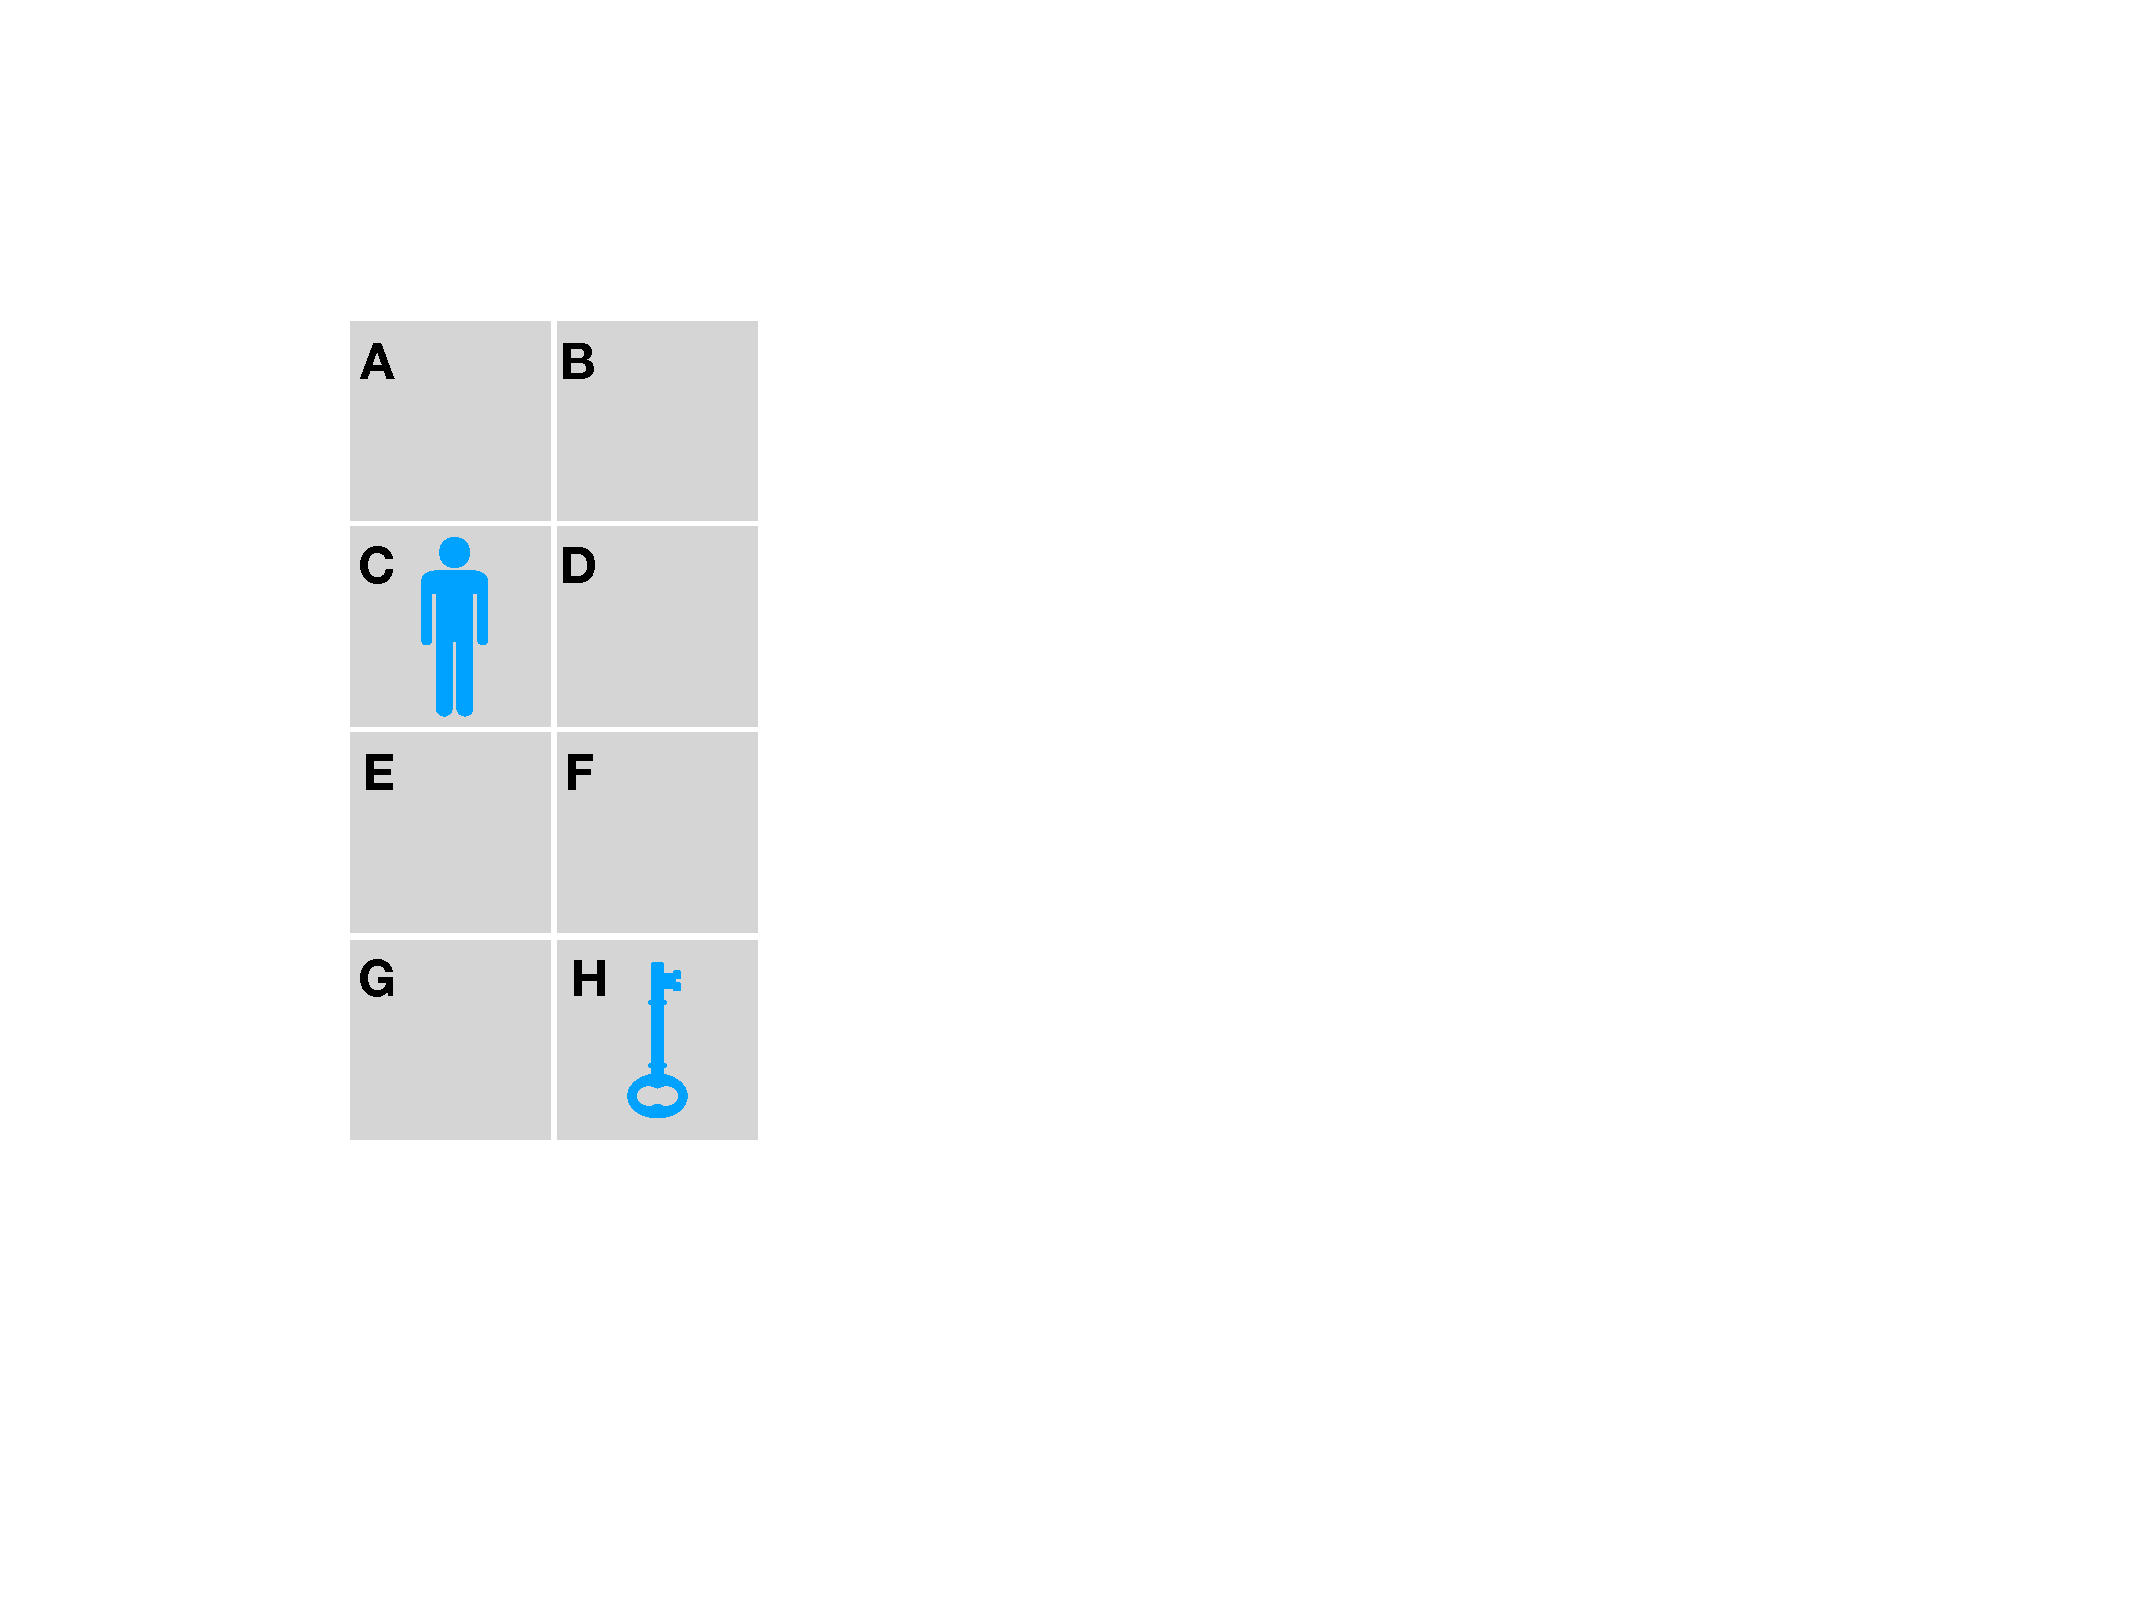
\includegraphics[width=0.15\textwidth]{figures/simple_nodir.pdf}
\label{fig:montezuma}
\end{center}



Order of nodes expanded:

Number of nodes expanded: 

Path returned: 

Length of path: 

Cost of path: 

What are $g(A), g(B), \ldots, g(H)$?

\def\arraystretch{1.5}
\setlength\tabcolsep{15pt}
\begin{center}
\begin{tabular}{|c|c|c|c|c|c|c|c|c|}
    \hline
      State $s$ & A & B & C & D & E & F & G & H  \\
    \hline
      $g(s)$ &  &  &  &  &  &  &  &  \\
    \hline
\end{tabular}
\end{center}

\end{subquestion}

\newpage
\begin{subquestion}[8]
\textbf{A* graph search (with Manhattan distance to the goal as the heuristic)}\\
Frontier data structure: priority queue (make sure you update/reorder the whole frontier after each addition)\\
Recall that A* computes $f(v)$ for the nodes $v$ that it expands, with $f(v) = g(v) + h(v)$ where $g(v)$ is the lowest cost to reach $v$ from the start node and $h(v)$ is an estimate of the distance from $v$ to the goal.\\

\begin{center}
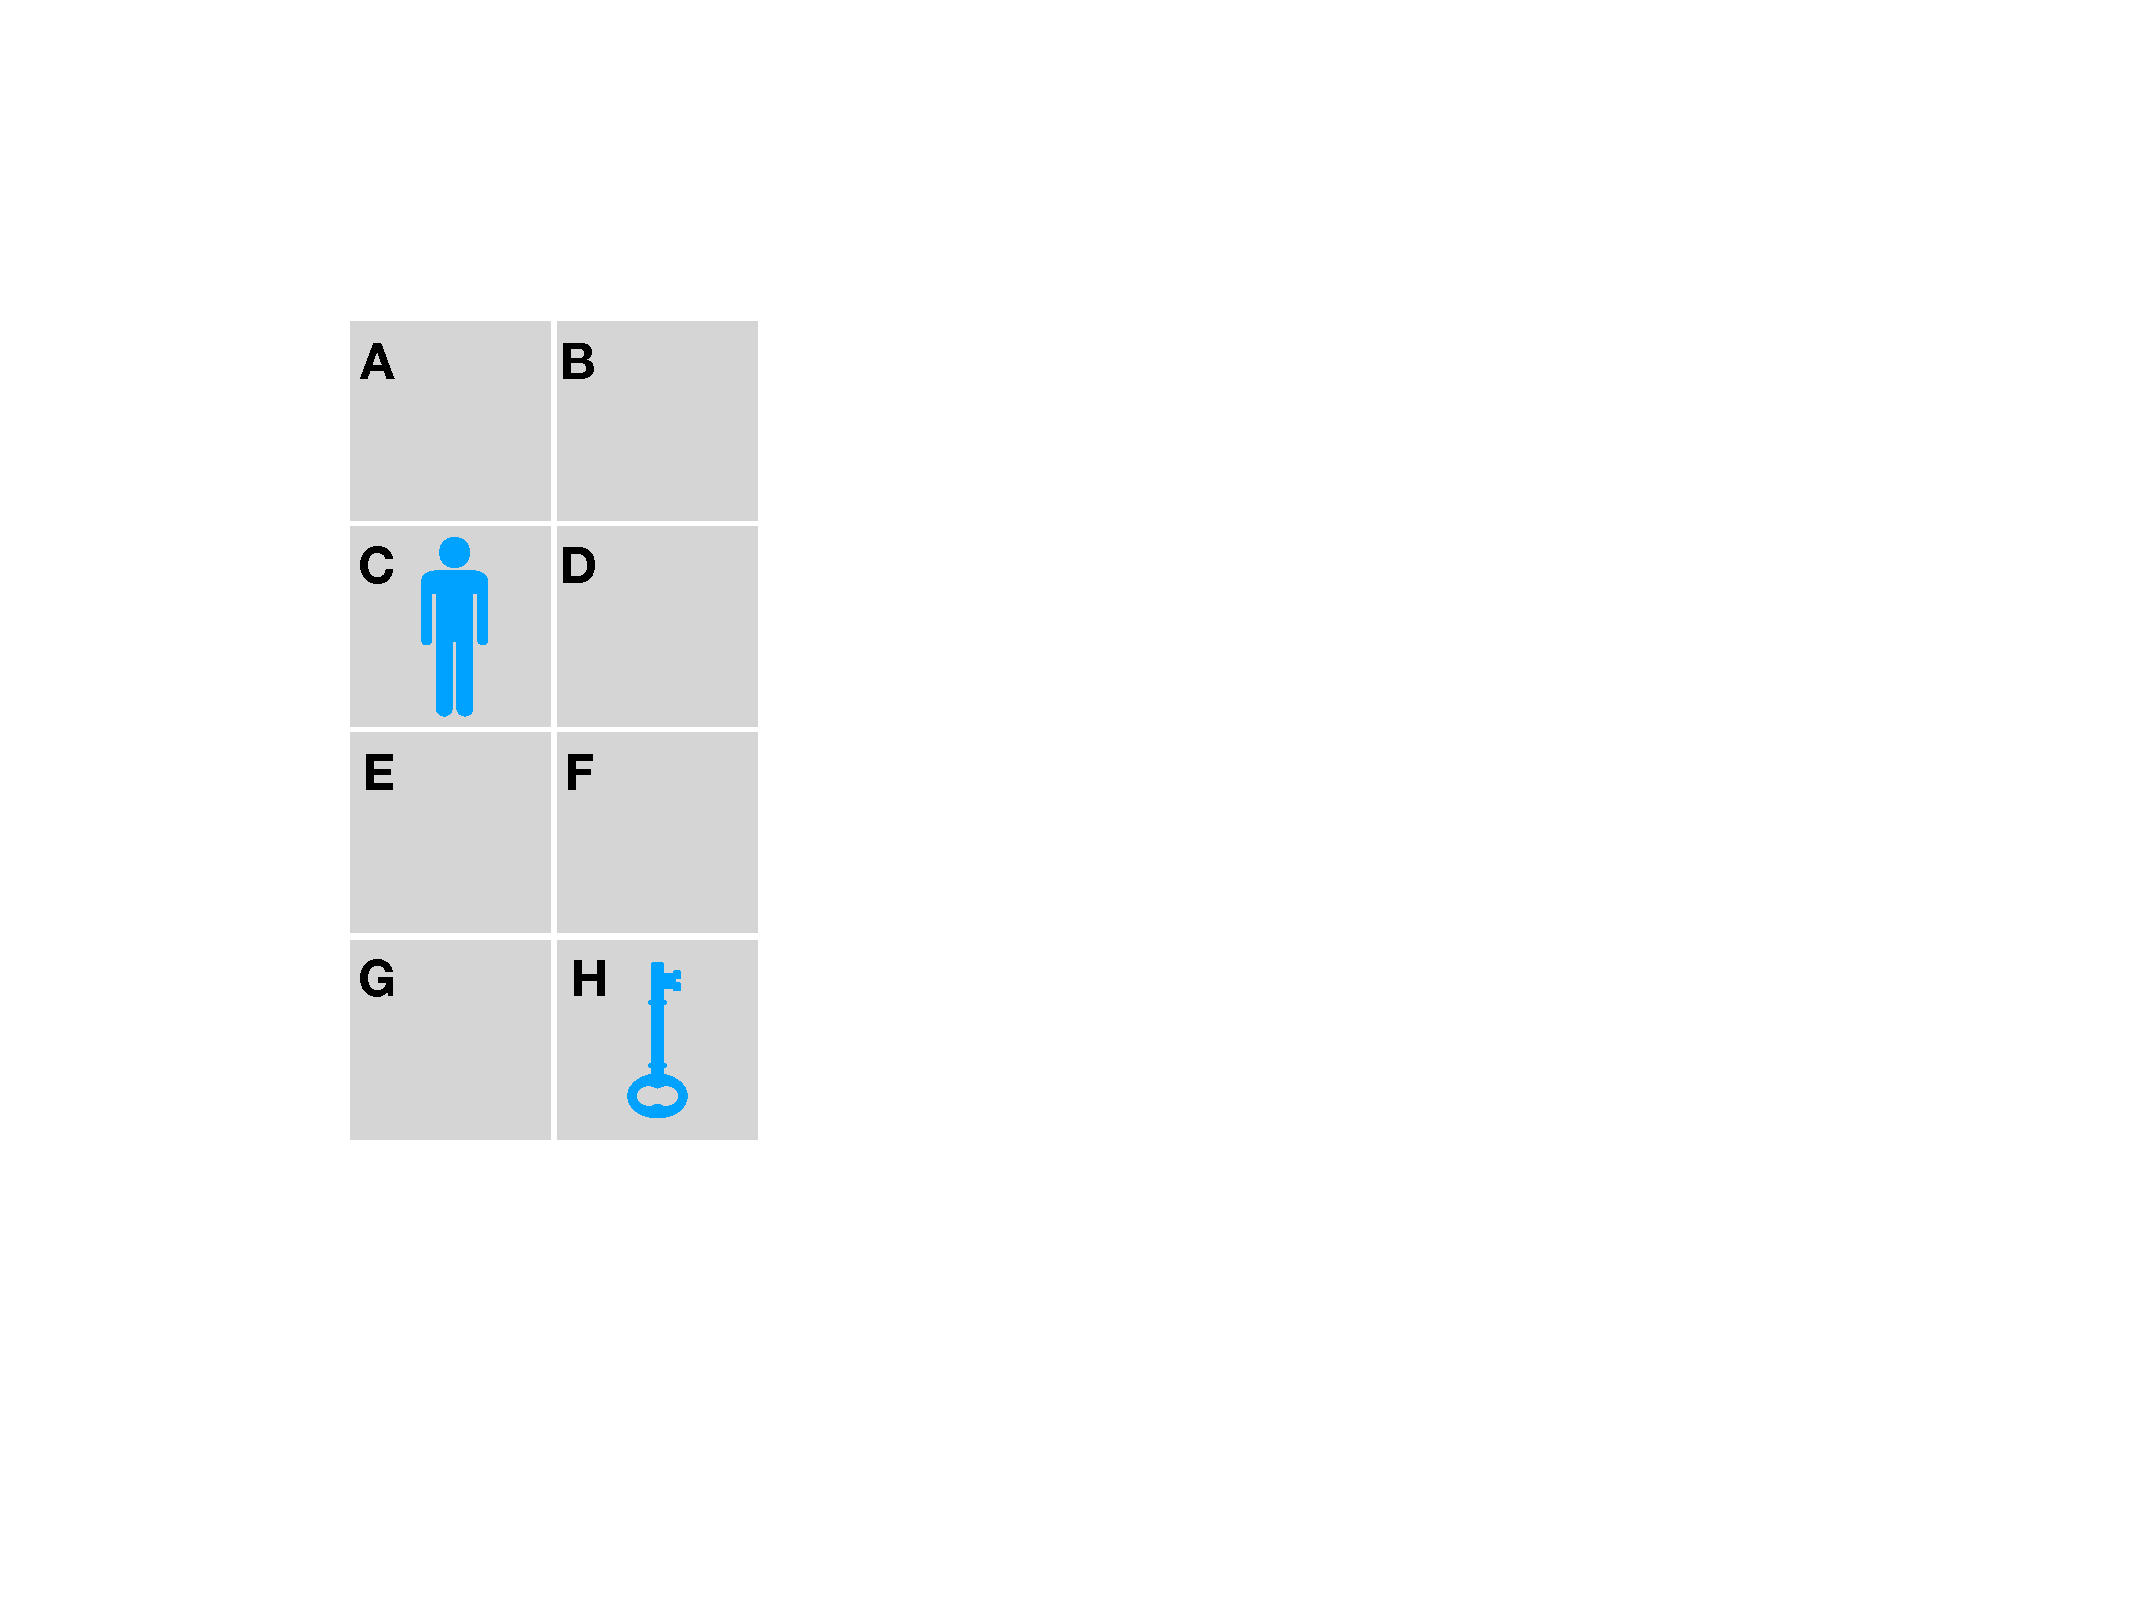
\includegraphics[width=0.15\textwidth]{figures/simple_nodir.pdf}
\label{fig:montezuma}
\end{center}



Order of nodes expanded during the search:

Number of nodes expanded during the search: 

Path returned by the search: 

Length of path returned by the search: 

Cost of path returned by the search: 

What are $f(A), f(B), \ldots, f(H)$? Note that the h(v) is found by calculating the Manhattan distance from v to goal. 
\\\\

\def\arraystretch{1.5}
\setlength\tabcolsep{15pt}
\begin{center}
\begin{tabular}{|c|c|c|c|c|c|c|c|c|}
    \hline
      State $s$ & A & B & C & D & E & F & G & H  \\
    \hline
      $f(s)$ &  &  &  &  &  &  &  &  \\
    \hline
\end{tabular}
\end{center}
\end{subquestion}

\end{question}

\newpage
\begin{question}[10]
Given your answers above, what are the qualitative differences between the results achieved by BFS, UCS, and A*? Which one finds the shortest path (in number of steps)? Which one finds the optimal path (in cost)?
\end{question}

\newpage
\begin{center}
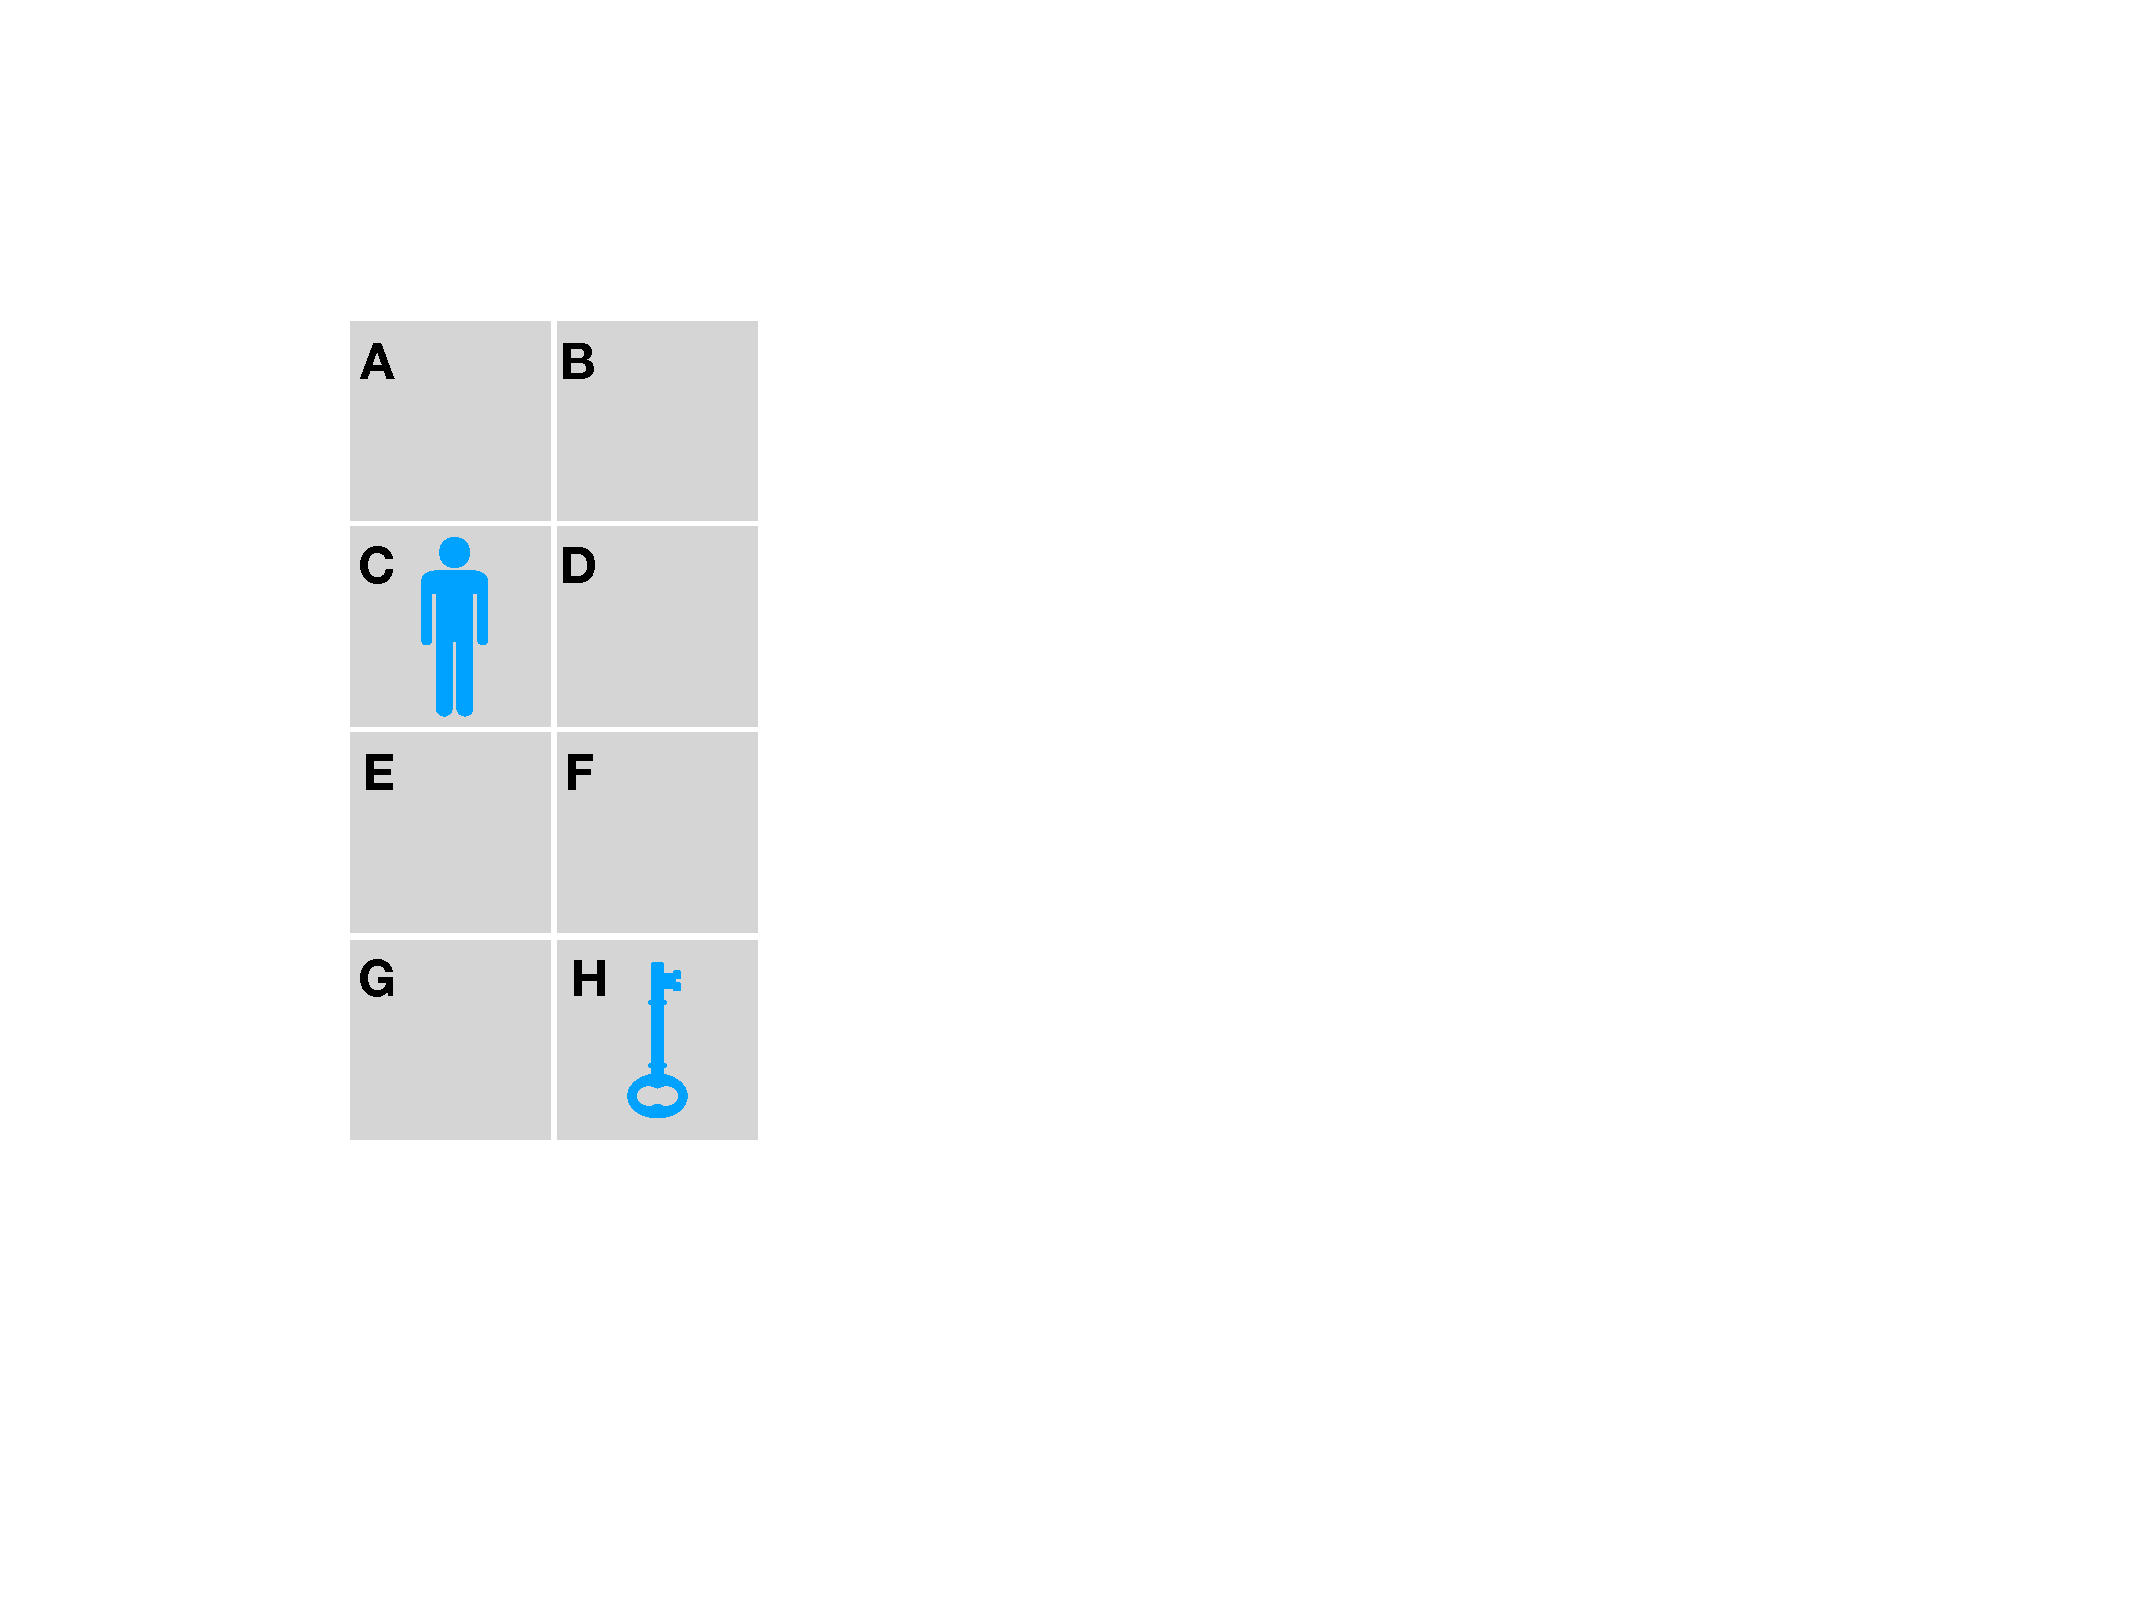
\includegraphics[width=0.15\textwidth]{figures/simple_nodir.pdf}
\end{center}

\begin{question}
For the same board and setting as part (b), give an example for each of the following types of heuristics. Please briefly explain why the example you chose satisfies the requested properties.

\begin{subquestion}[3]
Admissible and consistent. \\
Note: You can use a heuristic that we have frequently used in this class, or you can just assign any set of numbers to the states that qualifies as an admissible and consistent heuristic.

\def\arraystretch{1.5}
\setlength\tabcolsep{15pt}
\begin{center}
\begin{tabular}{|c|c|c|c|c|c|c|c|c|}
    \hline
      State $s$ & A & B & C & D & E & F & G & H  \\
    \hline
      Heuristic $h(s)$ &  &  &  &  &  &  &  &  \\
    \hline
\end{tabular}
\end{center}

Explanation: 

\end{subquestion}

\begin{subquestion}[4]
Admissible but inconsistent

\def\arraystretch{1.5}
\setlength\tabcolsep{15pt}
\begin{center}
\begin{tabular}{|c|c|c|c|c|c|c|c|c|}
    \hline
      State $s$ & A & B & C & D & E & F & G & H  \\
    \hline
       Heuristic $h(s)$ &  &  &  &  &  &  &  &  \\
    \hline
\end{tabular}
\end{center}

Explanation: 

\end{subquestion}

\begin{subquestion}[3]
Inadmissible and inconsistent

\def\arraystretch{1.5}
\setlength\tabcolsep{15pt}
\begin{center}
\begin{tabular}{|c|c|c|c|c|c|c|c|c|}
    \hline
      State $s$ & A & B & C & D & E & F & G & H  \\
    \hline
      Heuristic $h(s)$ &  &  &  &  &  &  &  &  \\
    \hline
\end{tabular}
\end{center}

Explanation: 

\end{subquestion}


\end{question}

\newpage
\begin{question}

\vspace{0.1in}


\begin{subquestion}[8]For this new version of the game, your friend Nancy suggests taking the old game setting from part (b) and now adding the ability for the agent to perform a maximum of one ``teleportation" action during the game. That is, on one of the agent's moves, it can choose to jump from its current state to any other non-goal state on the board, and the cost of teleporting is 1. \\


1. How does this new teleportation ability change the state space of the game from part (b), which was $(x,y)$? Does anything need to be added or removed?



2. Nancy argues that in this new game, at least one previously consistent heuristic can become inconsistent. Is Nancy right?

\mcqs Yes, and I will give an example below.\\
\mcqb No, and I will provide a proof below.\\

\textbf{Note:} we define heuristics for this problem as being a function of \textbf{only} the cell location: They cannot incorporate anything that did not exist in the old version of the game that we are comparing to.

\vspace{0.5em}
\hrulefill
\vspace{0.5em}

If you believe Nancy is right, give an example of a heuristic that used to be consistent in the old game but is no longer consistent in this new game. Make sure to explain why it is no longer consistent (perhaps with a drawing of a board state and an explanation). 


\def\arraystretch{1.5}
\setlength\tabcolsep{15pt}
\begin{center}
\begin{tabular}{|c|c|c|c|c|c|c|c|c|}
     \hline
State & A & B & C & D & E & F & G & H  \\
     \hline
      $h(s)$ &  &  &  &  &  &  &  &  \\
     \hline
 \end{tabular}
 \end{center}





\vspace{0.5em}
\hrulefill
\vspace{0.5em}


If you believe Nancy is wrong, provide an argument for why a heuristic that was consistent in the old game must also remain consistent in this new game. Be specific about your reasoning and use mathematical quantities such as heuristic costs of states $h(v)$ and true costs of actions $c(v,a,v')$.

\end{subquestion}

\newpage

\begin{subquestion}[8]For this new version of the board, your friend Ethan suggests adding the skull back to the old board setting from part (b), and having the skull move back and forth between the cells E and F. \\

1. How does the presence of this skull change the state space of the game from part (b), which was $(x,y)$? Does anything need to be added or removed?



2. Ethan argues that in this new board, at least one previously consistent heuristic can become inconsistent. Is Ethan right?\\

\mcqb Yes, and I will give an example below.\\

\mcqs No, and I will provide a proof below.\\

\textbf{Note:} we define heuristics for this problem as being a function of \textbf{only} the cell location: They cannot incorporate the location of the skull, since that did not exist in the old version of the board that we are comparing to.

\vspace{0.5em}
\hrulefill
\vspace{0.5em}

If you believe Ethan is right, give an example of a heuristic that used to be consistent on the old board but is no longer consistent on this new board. Make sure to explain why it is no longer consistent (perhaps with a drawing of a board state and an explanation. 

\def\arraystretch{1.5}
\setlength\tabcolsep{15pt}
\begin{center}
\begin{tabular}{|c|c|c|c|c|c|c|c|c|}
    \hline
      State & A & B & C & D & E & F & G & H  \\
    \hline
      $h(s)$ &  &  &  &  &  &  &  &  \\
    \hline
\end{tabular}
\end{center}



\vspace{0.5em}
\hrulefill
\vspace{0.5em}


If you believe Ethan is wrong, provide an argument for why a heuristic that was consistent in the old board must also remain consistent in this new board. Be specific about your reasoning and use mathematical quantities such as heuristic costs of states $h(v)$ and true costs of actions $c(v,a,v')$.


\end{subquestion}


\end{question}

\end{problem}